\title{Nektar++ Tutorial}



\documentclass[12pt]{article}
\usepackage{tikz}
\usepackage[lined,algo2e,boxed]{algorithm2e}
\begin{document}
\maketitle

\noindent
The aim of this tutorial is to lead the user through the \emph{Nektar++} features. The starting point is to compile the libraries, the solvers and the utilities
as explained on the website\footnote{www.nektar.info} . Once we are sure that everything is compiled we can run the regression tests to check that the software is producing the expected results and is working properly.\\

\noindent
In this document we will show how to create a simple 2D mesh using $Gmsh$ and how to convert the mesh file into the proper input format for \emph{Nektar++}.
Subsequently we will use this mesh to solve various problems:
\begin{enumerate}
\item the Helmholtz equation,
\item the Unsteady Advection-Diffusion equation,
\item and, in the end, the Incompressible Navier-Stokes equations. 
\end{enumerate}

\noindent
This approach should help the user to understand how in \emph{Nektar++}  we can specify the domain (mesh) where we want to solve a set of equations and
the equation itself.

\noindent
The last step of the tutorial is an example of a more complex fluid dynamics problem, the flow past a cylinder. The point of presenting this typical problem is to introduce some
more advanced features including the definition of curved elements and the restart files. 

\section{Geometry and Mesh}

We start creating a very simple geometry. A square which we will mesh with 16 quadrilateral elements.
The square is of size $[-\pi/2,\pi/2]\times[-\pi/2,\pi/2]$.\\

\noindent
If you look into the folder \emph{NekTutorial/Tutorial/SquareMesh/Geometry/}  you can find the following files
\begin{itemize}
\item $Square.geo$
\item $Square.msh$
\item $Square.xml$\\
\end{itemize}

\noindent
$Square.geo$ is the file containing the geometry and the instructions for $Gmsh$ to generate the mesh. $Square.msh$ is the output of $Gmsh$.
$Square.xml$ is the input file for \emph{Nektar++} without any definitions about the equation we want to solve over the domain.
If you want, you can generate the $.msh$ file from the terminal as

\vspace{5mm}
\begin{algorithm2e}[H]
gmsh -2 Square.geo
\end{algorithm2e}
\vspace{5mm}


\noindent
$Square.xml$ has been generated using the Preprocessing tools in the utilities folder.
To generate a $.xml$ file starting from a $.msh$ file you have just to call the $MeshConvert$ executable located in \emph{utilities/builds/PreProcessing/}
from the terminal as

\vspace{5mm}
\begin{algorithm2e}[H]
./MeshConvert Square.msh Square.xml
\end{algorithm2e}
\vspace{5mm}

Figure \ref{fig:Mesh} shows the domain over which we are going to solve our equations.

\begin{figure}
\centering
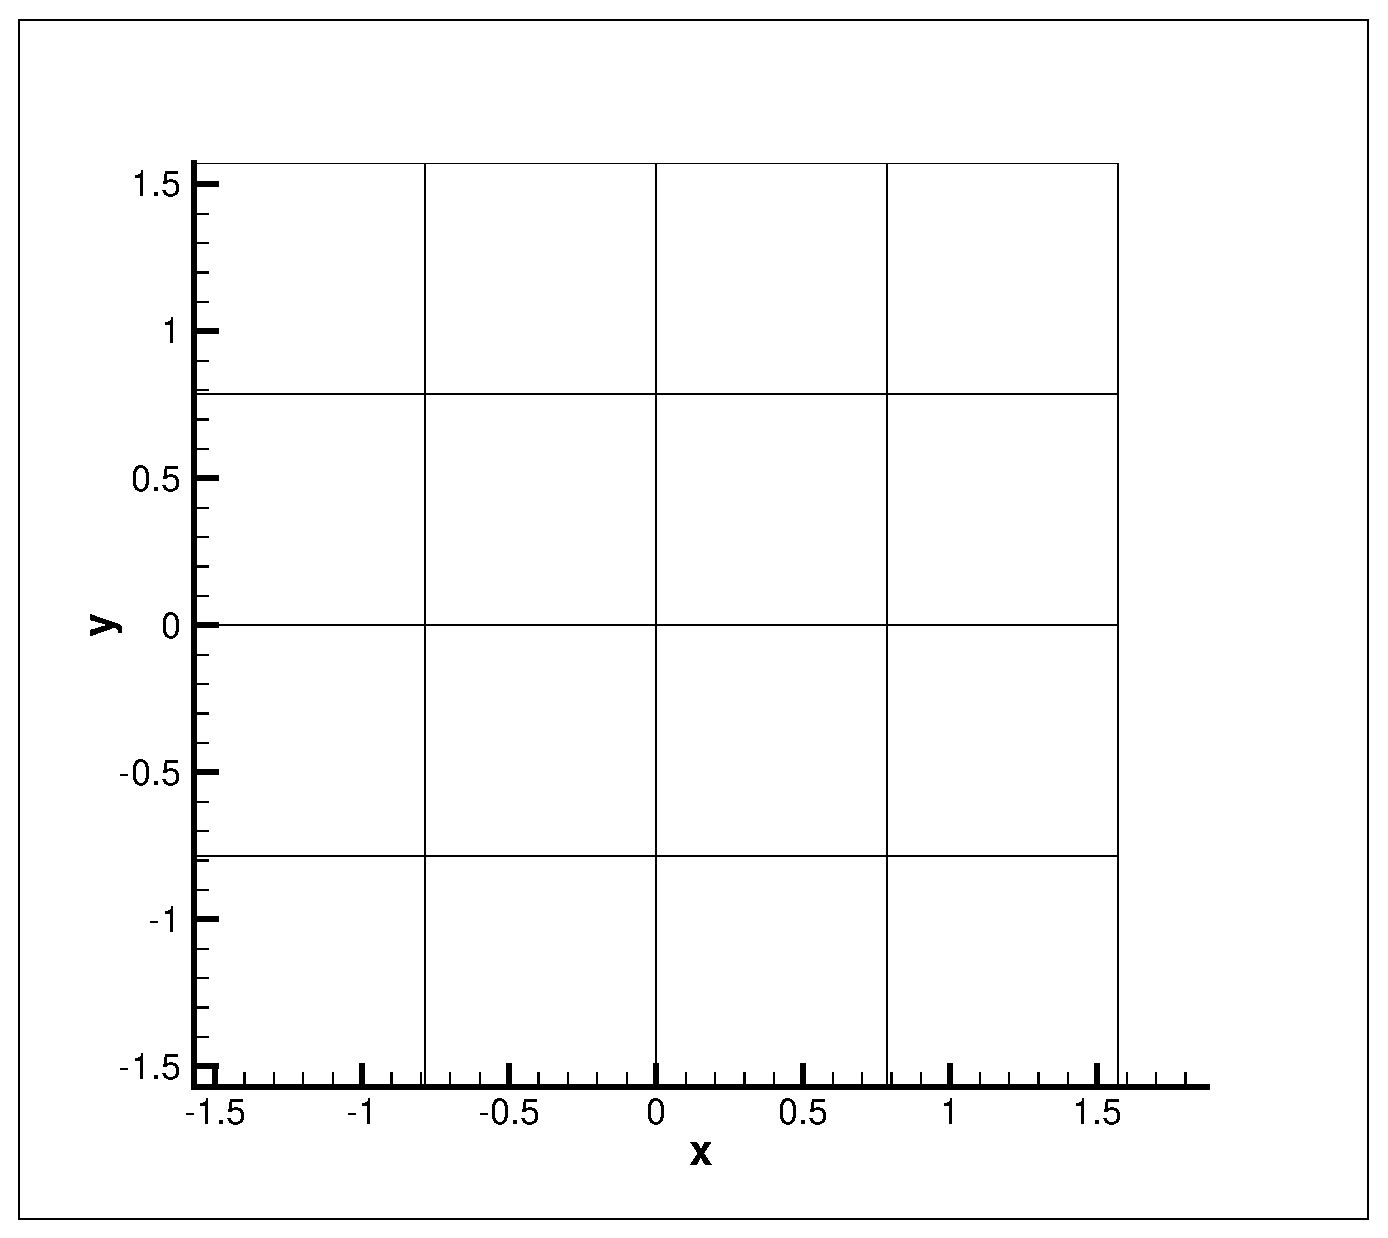
\includegraphics[scale=0.35]{mesh.eps}
\caption{16 quadrilaterals mesh}
\label{fig:Mesh}
\end{figure}

\section{Helmholtz equation}

We first want to solve the 2D Helmholtz equation on the domain we have just created; the equation is:
\begin{equation}
\nabla^2 u + \lambda u = f \quad u(x,y) \in \Omega
 \end{equation}
 \begin{equation}
f(x,y)= -(\lambda + 2\pi^2)\sin(\pi x)\sin(\pi y)
 \end{equation}
\begin{equation}
u_{ex}(x,y)= \sin(\pi x)\sin(\pi y)
 \end{equation}
 
 \noindent
 Into the folder \emph{NekTutorial/Tutorial/SquareMesh/Helmholtz/} you can find the following files
 \begin{itemize}
 \item $Test\_HEL.xml$, which is the $.xml$ already prepared to use the geometry and solve the problem;
 \item $Test\_HEL.fld$, which is the solution obtained with \emph{Nektar++};
 \item $Test\_HEL\_u.pos$, which is the file you can load in $Gmesh$ to see the solution.
 \end{itemize} 

\noindent
If we take a look of the  $Test\_HEL.xml$, we can see how we can define:
\begin{enumerate}

\item  the expansion type and order,\\
\vspace{5mm}
\begin{algorithm2e}[H]
EXPANSIONS \\\
    E COMPOSITE="C[0]" NUMMODES="8" TYPE="MODIFIED" \\
EXPANSIONS\\
 \end{algorithm2e}

\item the equation type, the projection type (Continous corresponds to the continuos Galerkin) and the parameters we need,\\    
\vspace{5mm}
\begin{algorithm2e}[H]
SOLVERINFO\\\
     PROPERTY="EQTYPE" VALUE="Helmholtz"\\\
     PROPERTY="Projection" VALUE="Continuous"\\
SOLVERINFO\\

PARAMETERS\\\
    wavefreq       = PI \\\
     Lambda        = 1.0\\
PARAMETERS
 \end{algorithm2e}

\item the variable/s declaration and the boundary regions linking to the defined geometry,\\    
\vspace{5mm}
\begin{algorithm2e}[H]
VARIABLES\\\
     ID="0" u \\ 
VARIABLES\\

BOUNDARYREGIONS\\\
    ID="0" C[1] \\
BOUNDARYREGIONS\\
\end{algorithm2e}

\item the definition of the boundary condition value (in this case we have used the exact solution as a Dirichlet boundary condition), the definition of the forcing term and the exact solution,\\
\vspace{5mm}
\begin{algorithm2e}[H]
BOUNDARYCONDITIONS\\\
         REGION REF="0"\\\
            D VAR="u" VALUE="sin(PI*x)*sin(PI*y)" \\\
         REGION\\
 BOUNDARYCONDITIONS\\
    
    FORCING\\\
      F VAR="u" VALUE="-(Lambda + 2*PI*PI)*sin(PI*x)*sin(PI*y)" \\
    FORCING\\
       
    EXACTSOLUTION\\\
      F VAR="u" VALUE="sin(PI*x)*sin(PI*y)" \\
    EXACTSOLUTION\\
\end{algorithm2e}
\end{enumerate}

\noindent            
The Helmholtz equation is then solved with the executable $ADRSolver$\footnote{ADRSolver has been design to solve all the problems derived from a typical Advection-Diffusion-Reaction equation. Switching the EQTYPE flag to another value and providing the proper information you can solve for example Poisson, Laplace, Steady/Unsteady Diffusion, Steady/Unsteady Advection, etc.}.
The executable is located in the folder \emph{solver/builds/dist/bin/}\footnote{Depending on the compilation mode you can find: ADRSolver, if you have compiled the solvers in Release mode, or ADRSolver-g, if you have compiled the solvers in Debug mode.}

\vspace{5mm}
\begin{algorithm2e}[H]
./ADRSolver Test\_HEL.xml
\end{algorithm2e}
\vspace{5mm}

\noindent
To produce the output for $Gmesh$ you need to use the $PostProcessing$ tools in the folder $utilities$, as we have done for the $PreProcessing$.
You can produce outputs for $Gmesh$, $TecPlot$ and $Paraview$ using the related converter from the terminal. For example for $Gmsh$ is

 \vspace{5mm}
\begin{algorithm2e}[H]
./FldToGmsh Test\_HEL.xml Test\_HEL.fld 
\end{algorithm2e}
\vspace{5mm}

\noindent
This executable will produce $Test\_HEL\_u.pos$ that can be loaded in $Gmsh$.

\section{Unsteady Advection-Diffusion equation}

Using the same mesh, we are going to solve now an Unsteady-Advection-Diffusion problem. As before for the Helmholtz problem, the files are located in
\emph{NekTutorial/Tutorial/SquareMesh/UnsAdvDiffusion/}. Here you can find the same kind of files which has been presented for the Helmholtz problem.

The equation we are solving is
\begin{equation}
\frac{\partial u}{\partial t} + V_X \frac{\partial u}{\partial x} + V_Y \frac{\partial u}{\partial y} = \epsilon \nabla^2 u
\end{equation}

\noindent
Setting $\epsilon = 1$ and $V_X=V_Y=0$ the exact solution is trivial and we can use it to set Dirichlet boundary condition on the edges.

\begin{equation}
u_{ex}= e^{-2\pi^2 t}\sin(\pi x)\cos(\pi y)
\end{equation}

\noindent
In this case the executable is still the $ADRSolver$ but we need to provide some more information to the input files, like the initial conditions and the time-integration parameters.

\vspace{5mm}
\begin{algorithm2e}[H]
SOLVERINFO\\\
        PROPERTY="EQTYPE" VALUE="UnsteadyAdvectionDiffusion" \\\
        PROPERTY="Projection" VALUE="Continuous"\\\
        PROPERTY="DiffusionAdvancement" VALUE="Implicit"\\\
        PROPERTY="AdvectionAdvancement" VALUE="Explicit"\\\
        PROPERTY="TimeIntegrationMethod" VALUE="IMEXOrder2"\\
SOLVERINFO\\
\end{algorithm2e}
\begin{algorithm2e}[H]
PARAMETERS\\\
      TimeStep      = 0.00001 \\\  
      NumSteps      = 2000\\\                
      IO\_CheckSteps = 2000\\\                 
      IO\_InfoSteps  = 2000\\\                 
      wavefreq = PI\\\                      
      epsilon = 1.0\\                       
 PARAMETERS\\
\end{algorithm2e}
\begin{algorithm2e}[H]
USERDEFINEDEQNS\\\
       F LHS="Vx" VALUE="0.0" \\\
       F LHS="Vy" VALUE="0.0"\\
USERDEFINEDEQNS\\
 \end{algorithm2e}
\begin{algorithm2e}[H]
 INITIALCONDITIONS\\\
        F VAR="u" VALUE="sin(wavefreq*x)*cos(wavefreq*y)" \\
    INITIALCONDITIONS\\
    \end{algorithm2e}
\vspace{5mm}

\section{Incompressible Navier-Stokes equations}

Again, using the same mesh, we can solve the Incompressible Navier-Stokes equations. In this case the executable in not the $ADRSolver$ anymore, but the $IncNavierStokesSolver$, which is located in the same folder of the previous one.\footnote{As for the ADRSolver we can have the Release and the Debug version.} All the files, as for the previous examples, are located in \emph{NekTutorial/Tutorial/SquareMesh/IncNavStokes/}.


\noindent
Considering an incompressible, isothermal flow with constant density and viscosity, the governing equations are the Navier-Stokes (NS) coupled to a velocity divergence-free constraint. In terms of primitive variables $(V,p)$, the variational formulation is written as
\begin{equation}
\frac{\partial V}{\partial t} + V \cdot  \nabla V = -\nabla p + \nu \nabla^2 V
\label{eq:NS1}
\end{equation}
\begin{equation}
\nabla \cdot V = 0
\label{eq:NSequation}
\end{equation}
where $p(x,t)$ is the kinematic pressure field and $\nu$ is the kinematic viscosity. The flow we are going to solve is the Taylor decaying vortex described by the following equations

\begin{equation}
u=-\cos(x)\sin(y)e^{-2t/Re}
\label{eq:Dec1}
\end{equation}
\begin{equation}
v=\sin(x)\cos(y)e^{-2t/Re}
\label{eq:Dec2}
\end{equation}
\begin{equation}
p=-\frac{1}{4}\Bigl(\cos(2x)+\cos(2y)\Bigr)e^{-4t/Re}
\label{eq:Dec3}
\end{equation}

\noindent
In this case we define 3 variables: the 2 velocity components and the pressure.

\begin{algorithm2e}[H]
    SOLVERINFO\\\
        I PROPERTY="EQTYPE" VALUE="UnsteadyNavierStokes"\\\
        I PROPERTY="AdvectionForm" VALUE="Convective"\\\
        I PROPERTY="TimeIntegrationMethod" VALUE="IMEXOrder1"\\
      SOLVERINFO
\end{algorithm2e}
\begin{algorithm2e}[H]
    PARAMETERS\\\
     TimeStep      = 0.00001\\\               
      NumSteps      = 1000 \\\                 
      IO\_CheckSteps = 1000\\\                  
      IO\_InfoSteps  = 1000\\\                 
      Kinvis        = 0.0001\\            
    PARAMETERS\\
  \end{algorithm2e}
   \begin{algorithm2e}[H]
    VARIABLES\\\
      V ID="0" u\\\  
      V ID="1" v\\\  
      V ID="2" p\\ 
    VARIABLES\\
  \end{algorithm2e}

\section{Flow past a cylinder}
Here a simulation of the two-dimensional flow past a circular cylinder in
a free stream.
This is an illustrative example of the use of \emph{Nektar++}
framework to solve more complex fluid dynamics problems
The solution, which highlights the vortex shedding, has been obtained using the $2^{nd}$
order stiffly stable splitting scheme with $\Delta t = 0.001 s$ and
$5^{th}$ order spectral/hp expansion on a mesh of $1500$
quadrilaterals. The cylinder has a diameter $D = 0.4$ and the domain
is defined by a rectangle $[-4\,,16] \times
[-5\,,5]$. Boundary conditions for the velocity filed
are of Dirichlet type at the inflow, where a constant velocity in
$x$-direction is imposed ($u = 1$ and $v = 0$) and of Neumann type
(homogeneous) at the outflow and on the upper and lower domain
limits. The pressure boundary conditions are of Neumann type at the inflow and on the upper and lower domain limits ($\partial p/\partial n = 0$). The pressure
value at the outflow has been set to zero (Dirichlet boundary  condition).\\

\noindent
In this case the solver is still the $IncNavierStokesSolver$ and all the files are stored in \emph{NekTutorial/Tutorial/VortexShedding/}.
In the $.xml$ file we can see how curved elements are defined in \emph{Nektar++} and how we can use a previous solution to initialise the flow.
As a matter of fact a $.rst$ file is actually a $.fld$ file obtained with \emph{Nektar++} and used to set the flow. In this case we want to start from a converged solution to speed
up the simulation.

\section{Extra examples}

In the folder \emph{NekTutorial/Tutorial/RegTests/}, you can find plenty of examples which are directly taken from the regression tests.

\end{document}
